\documentclass[11pt]{article}
% uncomment to set the page format to A4 instead of A5
\def\RELEASEDOCUMENT{}

% Change caption size
\usepackage[font = {footnotesize}]{caption}

% Preamble
% language and encoding
\usepackage[utf8]{inputenc}
\usepackage[T1]{fontenc}
\usepackage[brazil]{babel}

% fonts: normal and monospaced
%\usepackage[charter]{mathdesign}
\usepackage{mathpazo}
%\usepackage{newtxtext, newtxmath}
%\usepackage[scaled]{ulgothic}
\usepackage{inconsolata}

% page format
\ifdefined\RELEASEDOCUMENT
\usepackage[a4paper, margin=2cm]{geometry}
\else
\usepackage[a5paper, margin=1.5cm]{geometry}
\fi

% additional commands to math mode
\usepackage{amsmath}

% indent first line of first paragraph
\usepackage{indentfirst}

% page numbering
\pagestyle{empty}

% automatically format quotes (no need to write as ``'')
\usepackage{csquotes}
\MakeOuterQuote{"}


% support coloured links, PDF bookmarks, etc.
%\usepackage[colorlinks=false, pdfstartview=FitH, pdfpagelayout=OneColumn]{hyperref}

% remove space after a comma when it acts like a decimal separator
\usepackage{icomma}

% "cancel" terms with a slash
%\usepackage{cancel}

% enable use of colours
%\usepackage{xcolor}

% show customised enumerate 
%\usepackage{enumerate}

% support graphics
%\usepackage{graphicx}

% input raw text
%\usepackage{verbatim}

% add cells that span more than one row or column
%\usepackage{multirow, multicol}

% include external raw PDF pages
%\usepackage{pdfpages}

% allow forcing force a figure to be displayed "here"
%\usepackage{float}

% input code
%\usepackage{listings} \lstset{basicstyle=\ttfamily}

% add "lorem ipsum" text
\usepackage{blindtext} \blindmathtrue

% add questions and answers
\usepackage[]{exercise}
\renewcommand{\ExerciseName}{Questão}
\renewcommand{\ExerciseListName}{Q\!\!}
\renewcommand{\AnswerName}{Resposta}
\renewcommand{\AnswerListName}{Resposta}
\renewcommand{\ExePartName}{Item}
\renewcommand{\ExerciseHeader}{\hrule~\par\noindent{\textbf{\large
            \ExerciseName~\ExerciseHeaderNB\ExerciseHeaderTitle
            \ExerciseHeaderOrigin. \medskip}}}
\renewcommand{\ExePartHeader}{~\par\noindent{\textit{\large
            (\ExePartHeaderNB)
            \smallskip}}}
\renewcommand{\theExePart}{\alph{ExePart}}
\renewcommand{\ExePartHeaderNB}{\theExePart}



% add Portuguese trig functions
\DeclareMathOperator{\sen}{sen}
\DeclareMathOperator{\tg}{tg}
\DeclareMathOperator{\cotg}{cotg}
\DeclareMathOperator{\cossec}{cossec}
\DeclareMathOperator{\arcsen}{arcsen}
\DeclareMathOperator{\arctg}{arctg}
\DeclareMathOperator{\arccotg}{arccotg}
\DeclareMathOperator{\arccossec}{arccossec}

% add British commands and environments
\newenvironment{centre}[0]{\begin{center}}{\end{center}}
\newenvironment{itemise}[0]{\begin{itemize}}{\end{itemize}}


% Bibliography
\usepackage[backend = bibtex, sorting = none]{biblatex}
\renewbibmacro{in:}{}
\bibliography{referencias}{}
\urlstyle{same} % don't write URLs in monospaced font

% Custom title features
\usepackage{titling}

\def\thecourse{MAC0412 --- Organização de Computadores}
\def\theprofessor{Professor: Siang Wun Song}
\def\theinstitution{
    Instituto de Matemática e Estatística\\
    Universidade de São Paulo
}
\title{Computação em Nuvem}
\author{
    Leonardo Pereira Macedo   --- 8536065\\
    Vinícius Bitencourt Matos --- 8536221
}

\date{Dezembro de 2015}

% Add metadata to PDF
\hypersetup{
    pdfauthor = {Leonardo Pereira Macedo e Vinícius Bitencourt Matos},
    pdftitle = {\thetitle},
    pdfsubject = {Monografia para a disciplina Organização de Computadores},
    pdfpagemode = UseOutlines
}


\begin{document}

% prevent lines from going over margins
\sloppy

% add cover and table of contents to PDF bookmarks
\pdfbookmark[1]{Capa}{title} 


\begin{titlepage}
    \begin{center}
        \large\theinstitution
        \\\vfill
        \Huge\thetitle
        \\\vfill
        \LARGE\thecourse\\
              \theprofessor
        \\\vfill
        \Large\theauthor
        \\
        \vfill
        \Large\thedate
    \end{center}
\end{titlepage}
\setcounter{page}{2}
\pdfbookmark[1]{Sumário}{toc}
\tableofcontents 
\clearpage

\section{Introdução}

O termo computação em nuvem, do inglês \emph{cloud computing}, refere-se à 
utilização da memória e das capacidades de armazenamento e cálculo de computadores e 
servidores compartilhados e interligados por meio da 
Internet~\cite{aun-usp-dropbox-cloud-computing}, seguindo o princípio da computação 
em grade (modelo computacional capaz de alcançar uma alta taxa de processamento 
dividindo as tarefas entre diversas máquinas, podendo ser em rede local ou rede de 
longa distância, que formam uma máquina virtual~\cite{ibm-redbooks-grid-computing}).

O armazenamento de dados é feito em serviços que podem ser acessados de qualquer 
lugar do mundo, a qualquer hora, não havendo necessidade de instalar programas ou de 
armazenar dados. O acesso a programas, serviços e arquivos é remoto, através da 
Internet --- daí a alusão à nuvem. O uso desse modelo (ambiente) é mais viável do 
que o uso de unidades físicas~\cite{aun-usp-dropbox-cloud-computing}.

Num sistema operacional disponível na Internet, a partir de qualquer computador e em 
qualquer lugar, pode-se ter acesso a informações, arquivos e programas num sistema 
único, independente de plataforma~\cite{aun-usp-dropbox-cloud-computing}. O 
requisito mínimo é um computador compatível com os recursos disponíveis na Internet.

Na prática, a computação em nuvem seria a transformação dos sistemas computacionais 
físicos de hoje em uma base virtual. Ela tem como principal característica a 
transformação do tradicional modo de se utilizar e adquirir os recursos da TI 
(\emph{Tecnologia da Informação}) pelas empresas. O processo todo resulta de uma 
longa transição da computação baseada em hardware para a computação baseada em 
software e agora na Web~\cite{reuters-industry-hope-clouds}. As nuvens permitem que 
recursos não utilizados de computação sejam compartilhados, ou "virtualizados", e 
reutilizados por outros clientes, o que maximiza a 
eficiência~\cite{reuters-industry-hope-clouds}. E para reduzir ainda mais os custos, 
a maioria desses sistemas funciona com software de código aberto, de baixo 
custo~\cite{reuters-industry-hope-clouds}.

O termo \textbf{computação em nuvem} é relativamente recente, mas se analisarmos bem,
veremos que a ideia não é necessariamente nova. Já existem alguns serviços que,
de certa forma, encaixam-se dentro do conceito de computação em nuvem. Abaixo estão
alguns exemplos:

\begin{itemise}
    \item E-mail (Gmail, Yahoo! Mail)

    \item Discos virtuais (Dropbox, Google Drive, OneDrive)

    \item Armazenamento e compartilhamento de fotos ou vídeos (Flickr, YouTube)
\end{itemise}

\section{Por que uma nuvem?}

Ao consultar livros de redes, telecomunicações e afins, é provável que sempre
encontremos desenhos de nuvens usados para fins de abstração. Nesse sentido, a
ilustração representa uma rede de algum tipo cuja estrutura não precisa ser
conhecida, pelo menos não naquele momento.

Se a intenção em determinado capítulo é explicar como funciona uma tecnologia de
comunicação que interliga duas redes de computadores, por exemplo, não é
necessário detalhar as características de cada uma delas. Assim, o autor pode
utilizar uma nuvem --- a abstração --- para indicar que há redes ali.

A computação em nuvem simplesmente absorveu essa ideia, até porque o desenho de
uma nuvem, no mesmo contexto de abstração, passou também a representar a
internet.

\begin{figure}[ht]
    \centering
    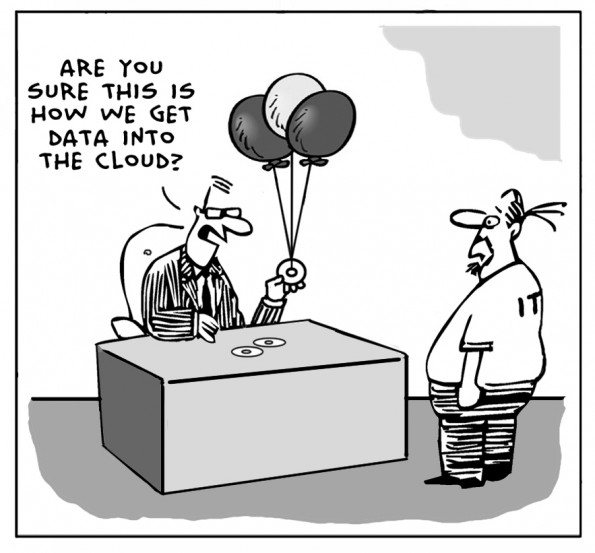
\includegraphics[width=0.3\textwidth]{img/comic.jpg}
    \caption{Charge retratando a "entrada de dados" na nuvem}
\end{figure}

\section{Um pouco de história}

Computação em nuvem não é um conceito claramente definido. Não estamos tratando de
uma tecnologia pronta que saiu dos laboratórios pelas mãos de um grupo de
pesquisadores e posteriormente foi disponibilizada no mercado. Essa característica
faz com que seja difícil identificar com precisão a sua origem. Mas há alguns
indícios bastante interessantes.

Um deles remete ao trabalho desenvolvido por John McCarthy, cientista da computação 
norte-americano conhecido como o "pai da IA" e o criador da linguagem Lisp. Na 
década de 1960, ele tratou de uma ideia bastante importante: computação por tempo 
compartilhado (\emph{time sharing}), em que um computador pode ser utilizado 
simultaneamente por dois ou mais usuários para a realização de determinadas tarefas, 
aproveitando especialmente o intervalo de tempo ocioso entre cada processo. Segundo 
McCarthy: "Computação poderá um dia ser organizada como uma utilidade pública assim 
como o telefone."~\cite{meersman2010move} Pagar-se-ia pelo que seria usado de fato. 
No entanto, a tecnologia da época não era poderosa o suficiente paa seguir essa 
ideia porque envolvia multiprogramação.

Na mesma época, o físico e cientista da computação Joseph Carl Robnett Licklider 
entrou para a história ao ser um dos pioneiros da Internet. Licklider, ao propor sua 
visão de uma \emph{Rede de Computadores 
Intergalática}~\cite{computerweekly-history-cloud-computing}, acabou sendo um dos 
primeiros a entender que os computadores poderiam ser usados de maneira conectada, 
de forma a permitir comunicação de maneira global e, consequentemente, o 
compartilhamento de dados.

Em 2006, o engenheiro de software norte-americano Eric Schmidt, da Google, 
popularizou o termo \emph{computação em nuvem} em uma palestra 
\cite{google-eric-schmidt} para descrever um novo paradigma, onde pessoas cada vez 
acessavam software e arquivos através da rede em vez de localmente em suas máquinas.

\begin{figure}[ht]
    \centering
    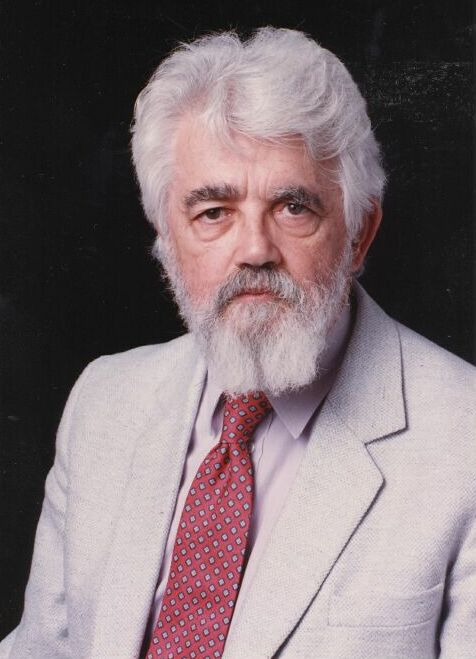
\includegraphics[height=0.3\textwidth]{img/mcCarthy.jpg}
    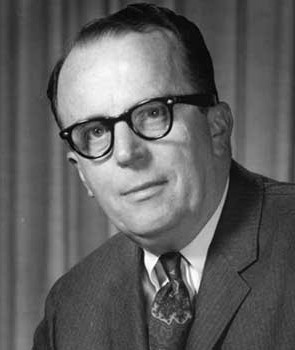
\includegraphics[height=0.3\textwidth]{img/licklider.jpg}
    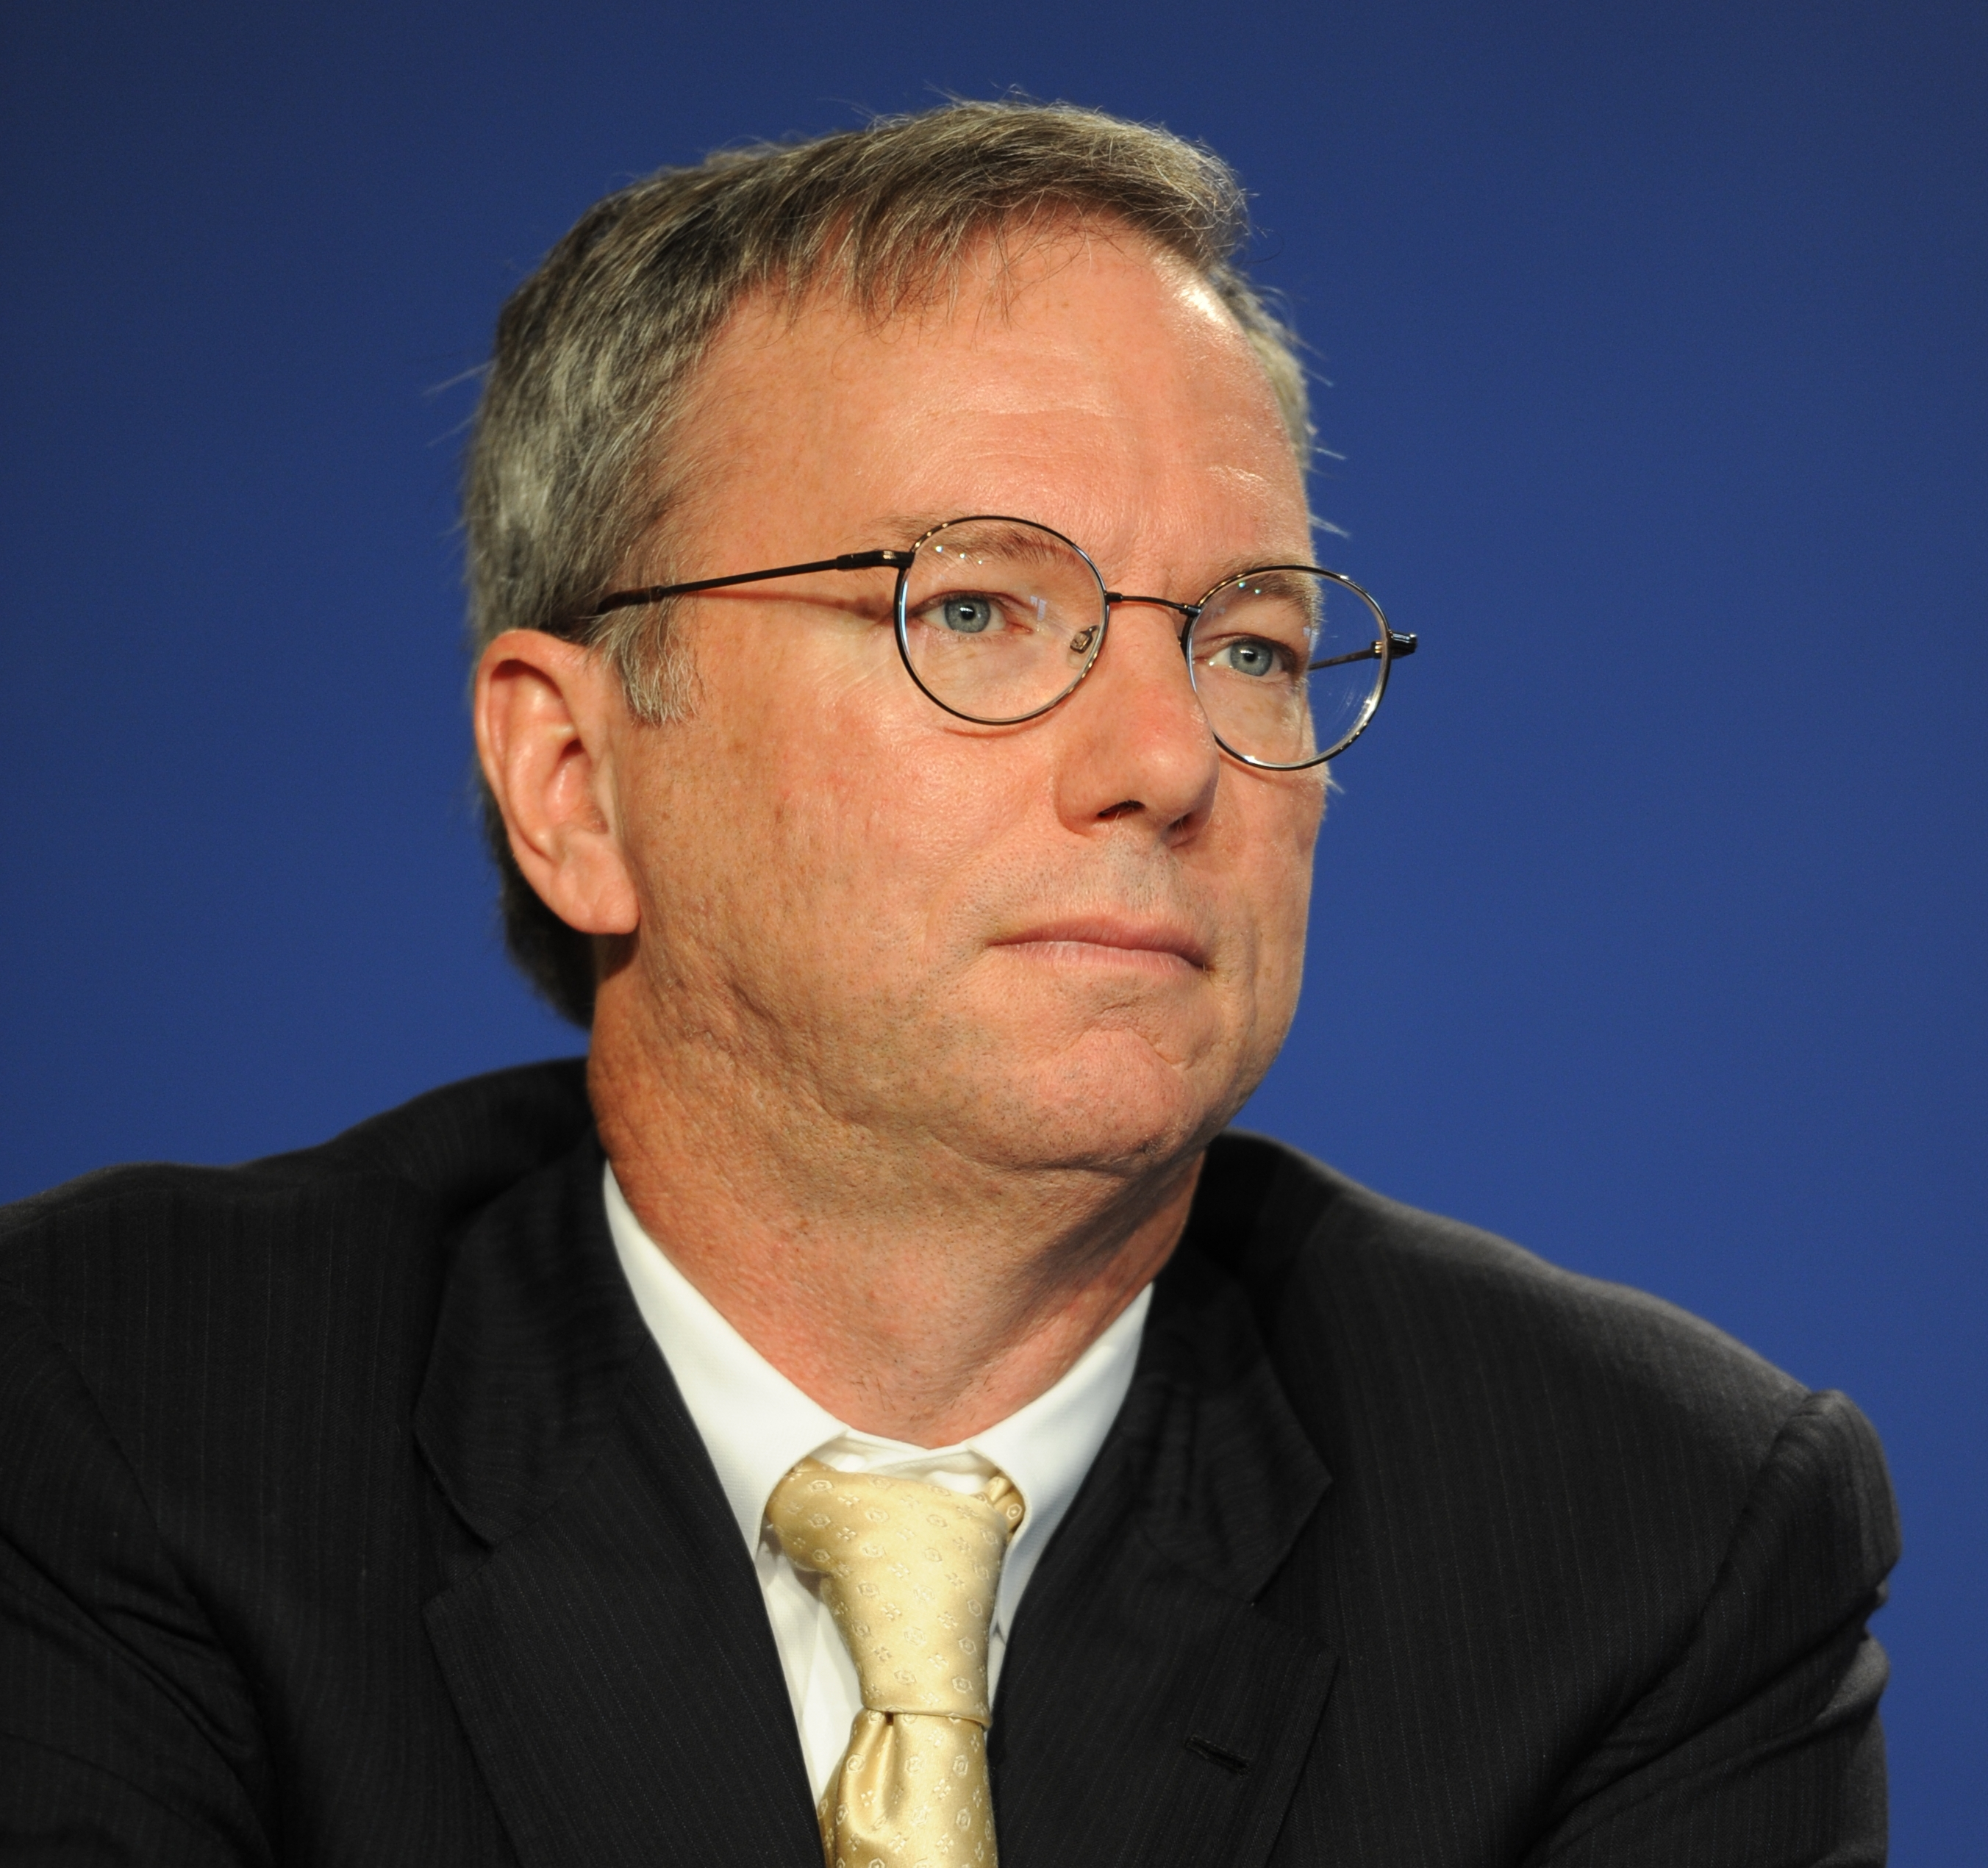
\includegraphics[height=0.3\textwidth]{img/schmidt.jpg}
    \caption{Da esquerda para a direta, John McCarthy~\cite{stanford-mccarthy-obit},
        J. C. R. Licklider~\cite{atimes-zoya-phantom} e Eric
        Schmidt~\cite{forbes-eric-schmidt:online}}
\end{figure}

% TODO: Mover, talvez, para a conclusão
% A computação em nuvem, até poucos anos atrás, era tida como uma tendência, mas hoje
% em dia é possível encontrar cada vez mais serviços que funcionam a partir de uma
% conexão com a Internet.

% Agora, fica a expectativa da evolução da computação em nuvem: por exemplo, será
% mesmo possível rodar todo um sistema operacional na nuvem? 

\section{Vantagens em se usar a nuvem}

Há razões válidas e significativas, de negócios e de TI, para as empresas transferirem
seus dados para trabalhar na nuvem. Os aspectos fundamentais são:

\newcommand{\itemm}[1]{\item\textbf{#1}}

\begin{itemise}
    \itemm{Redução de custo:} A computação em nuvem pode reduzir os custos de
        despesas de capital e despesas operacionais, pois os recursos só são adquiridos
        quando necessário, e só se paga por eles quando são usados. Ou seja, a necessidade
        de se investir em infrastrutura é menor.

    \itemm{Uso refinado da equipe:} Usar a computação em nuvem libera equipe de
        valor, permitindo que eles se concentrem em entregar valor, e não em manter
        hardware e software.

    \itemm {Escalabilidade robusta:} A computação em nuvem permite escala imediata,
        para mais ou para menos, a qualquer momento, sem compromisso a longo prazo.
        Por exemplo: se houvesse necessidade de ampliar um serviço de uma empresa, talvez
        fosse necessário comprar mais hardware. Com a computação em nuvem, essa escala
        é facilmente e rapidamente ajustada; basta adquirir mais espaço na nuvem.

\end{itemise}

Outras vantagens incluem maior segurança (requisito implementado por diversas companhias que
oferecem serviços de nuvem), organização (é possível controlar quais trabalhadores têm acesso
a quais arquivos) e flexibilidade de acesso (a nuvem pode ser acessada de qualquer lugar).

\undef\itemm

\section{Desvantagens em se usar a nuvem}

\subsection{Requisitos de largura da banda}

Ao adotar a estrutura de nuvem, a largura da banda e seu potencial gargalo devem ser 
considerados na estratégia. Segundo Bernard 
Golden~\cite{cio-cloud-computing-bottleneck}:

\begin{displayquote}
\emph{
    "Implementadores de virtualização descobriram que o principal gargalo para a 
    densidade de máquinas virtuais é a capacidade de memória. Agora, há um novo
    leque de servidores sendo lançados com áreas de cobertura da memória muito
    maiores, eliminando a memória como um gargalo do sistema. A computação em nuvem
    elimina esse gargalo removendo a questão da densidade de máquinas --- lidar com
    isso é responsabilidade do provedor da nuvem, fazendo com que o usuário não tenha
    com que se preocupar.
    Para a computação em nuvem, a largura da banda, de e para o provedor de nuvem,
    é um gargalo."
}
\end{displayquote}

\subsection{Problemas específicos}

Infelizmente, a nuvem também traz problemas para algumas empresas 
usarem-na~\cite{webhostblog-reasons-not-to-use-cloud}:

\newcommand{\itemm}[1]{\item\textbf{#1}}

\begin{itemise}

    \itemm{Tempo gasto para realizar a transição:} Uma empresa não pode migrar
    diretamente suas aplicações atuais para aplicações em nuvem. Isto requer
    personalização e tempo gasto em mover dados valiosos para aplicações mais
    amigáveis.

    \itemm{Surgimento de dificuldades durante a mudança:} O departamento de TI 
    precisa realizar a transição de monitoramento de hardware para monitorar o uso 
    de software. Tal procedimento pode levar a múltiplas alterações nas ferramentas 
    de gerenciamento, além da preocupação em garantir a estabilidade e 
    acessibilidade da nuvem a qualquer momento.

\end{itemise}

\undef\itemm

\section{Visão geral da arquitetura}

\newcommand{\frontend}{\emph{front-end}\xspace}
\newcommand{\backend} {\emph{back-end}\xspace}

A arquitetura da computação em nuvem é dividida geralmente em duas 
seções~\cite{rao-cloud-computing}, conectadas por meio de uma rede (geralmente a 
Internet):

\newcommand{\itemm}[1]{\item\textbf{#1}}

\begin{itemise}
    
    \itemm{Front-End:} É o lado visível ao cliente/usuário. Inclui o sistema ou rede
    de computador do cliente que é usada para acessar a rede. A interface é diferente
    dependendo do sistema de computação em nuvem (e-mail, etc.).

    \itemm{Back-End:} O lado usado pelo serviço oferecido, seria "a nuvem em si". 
    Inclui vários servidores, computadores, sistemas para armazenar dados, máquinas 
    virtuais... Juntas, elas constituem os serviços da computação em nuvem. O 
    \backend possui algumas responsabilidades para cumprir: implementar mecanismos 
    de segurança e controle de tráfego, e conectar computadores na rede para 
    comunicação através de protocolos (regras fixas e bem definidas).

\end{itemise}

\undef\itemm

\begin{figure}[ht]
    \centering
    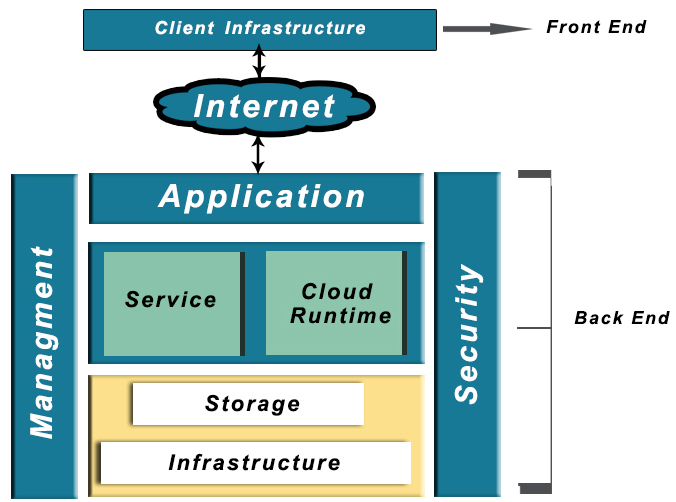
\includegraphics[width=0.5\textwidth]{img/frontBackEnd.jpg}
    \caption{Imagem retratando as duas seções principais da
        arquitetura~\cite{hostdepartment-overview-cloud}
    }
\end{figure}

\section{Topologia: Computação como uma mercadoria}

O conceito da nuvem é construído sobre camadas, cada uma fornecendo um nível
distinto de funcionalidade. Essa estratificação dos componentes forneceu o
meio para que as camadas da computação em nuvem se tornassem uma mercadoria, como
eletricidade, serviço telefônico ou gás natural. A mercadoria que a computação em
nuvem vende é poder computacional a um custo e despesas menores para o usuário.
Espera-se que a computação em nuvem se torne o próximo serviço megautilitário.

Como exemplo, explicaremos o \emph{Virtual Machine Monitor} (VMM) da IBM. Ele fornece o meio para
uso simultâneo das instalações de nuvem (figura \ref{fig:vmm}). VMM é um programa em
um sistema host que permite que um computador suporte diversos ambientes de execução
idênticos. Do ponto de vista do usuário, o sistema é um computador autocontido que
é isolado dos outros usuários. Na realidade, cada usuário está sendo servido pela
mesma máquina. Na computação em nuvem, o VMM permite que usuários monitorem e gerenciem
aspectos do processo, tais como acesso a dados, armazenamento de dados, criptografia,
endereçamento, topologia e movimento de carga de trabalho. 


\begin{figure}[ht]
    \centering
    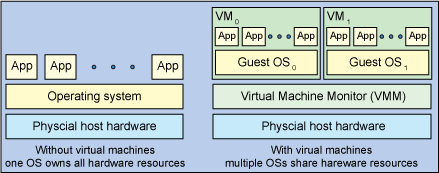
\includegraphics[width=0.6\textwidth]{img/vmm.png}
    \caption{Como o Virtual Machine Monitor funciona~\cite{cloud-computing-fundamentals}.}
    \label{fig:vmm}
\end{figure}


As camadas principais que a nuvem oferece são~\cite{cloud-computing-fundamentals}:

\newcommand{\itemm}[1]{\item\textbf{#1}}

\begin{itemise}

    \itemm{IaaS --- Infrastructure as a Service:} Camada que constitui a base da nuvem.
    Consiste nos ativos físicos --- servidores, dispositivos de rede, discos de armazenamento,
    etc. Ao usar IaaS, o cliente não controla de fato a infraestrutura subjacente, mas sim
    os sistemas operacionais, armazenamento, aplicativos de implementação e, até certo ponto,
    os componentes de rede selecionados. 

    Serviços de \emph{Print On Demand} (POD) são um exemplo de organizações que podem se
    beneficiar da IaaS. O modelo de POD é baseado na venda de produtos customizados, onde
    pessoas podem abrir lojas e vender designs de produtos. Os lojistas podem carregar
    o número de designs que quiserem à medida que os criam. Muitos carregam milhares.
    Com recursos de armazenamento em nuvem, um POD pode fornecer espaço de armazenamento
    ilimitado.

    \itemm{PaaS --- Plataform as a Service:} Camada intermediária. Fornece acesso a
    sistemas operacionais e serviços associados, além de uma maneira de implementar
    aplicativos para a nuvem usando linguagens de programação e ferramentas suportadas
    pelo fornecedor. Não é necessário gerenciar ou controlar a infraestrutura subjacente;
    o cliente tem controle dos aplicativos implementados e, até certo ponto, de configurações
    de ambiente de \emph{hosting} de aplicativos. 

    PaaS tem provedores como \emph{Elastic Compute Cloud} (EC2) da Amazon. A pequena 
empresa de software é um empreendimento ideal para PaaS. Com a plataforma elaborada,
produtos de classe mundial podem ser criados sem o gasto adicional da produção
interna.

    \itemm{SaaS --- Software as a Service:} É a camada superior (a de aplicativo), a qual
    a maioria visualiza como a nuvem. Aplicativos são executados aqui e são fornecidos
    sob demanda para os usuários. SaaS tem provedores como \emph{Google Pack}, que
    inclui aplicativos que podem ser acessados pela Internet, ferramentas como Gmail,
    Google Talk, Docs e outros.

\end{itemise}

\begin{figure}[H]
    \centering
    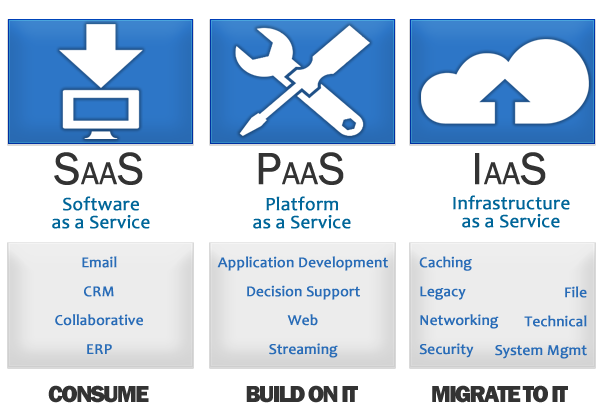
\includegraphics[width=0.5\textwidth]{img/services2.png}
    \caption{Principais camadas de computação em nuvem integradas nos componentes
        "como serviço"~\cite{cloud-computing-fundamentals}
    }
    \label{fig:layers}
\end{figure}


Existem também outros serviços oferecidos pela computação em 
nuvem~\cite{informatica}:

\begin{itemise}

    \itemm{DevaaS - Development as a Service:} As ferramentas de desenvolvimento tomam
    forma na computação em nuvem como ferramentas compartilhadas, ferramentas de
    desenvolvimento \emph{web-based} e serviços baseados em \emph{mashup}. 

    \itemm{CaaS - Communication as a Service:} Uso de uma solução de comunicação unificada
    hospedada em data center do provedor ou fabricante (exemplo: Microsoft Lync). 

    \itemm{EaaS - Everything as a Service:} Quando tudo é utilizado: infraestrurura,
    plataformas, software, suporte... Enfim, o que envolve Tecnologia da Informação e
    Comunicação como um serviço. 

    \itemm{DBaas - Database as a Service:} Quando a parte de servidores de banco de dados
    é utilizada como serviço.

    \itemm{TaaS - Testing as a Service:}: Oferece um ambiente apropriado para que o usuário
    possa testar aplicações e sistemas de maneira remota, simulando o comportamento destes
    em nível de execução.

\end{itemise}

\undef\itemm

% \begin{figure}[ht]
%     \centering
%     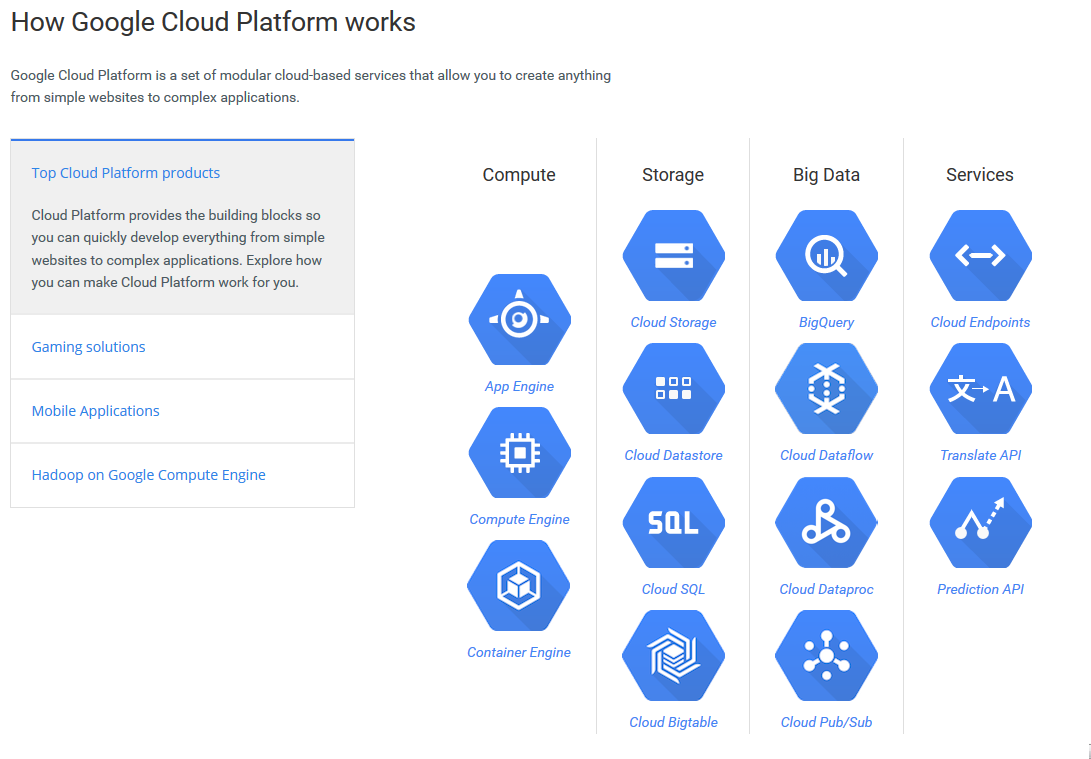
\includegraphics[width=0.8\textwidth]{img/googlecloud.png}
%     \caption{Exemplo do provedor
%              \href{https://cloud.google.com/}{Google~Cloud~Platform}
%              para os serviços oferecidos para computação em nuvem
%             }
%     \label{img:googlecloud}
% \end{figure}

\section{Modelo de implantação}

No modelo de implantação, dependemos das necessidades das aplicações que serão
implementadas. A restrição ou abertura de acesso depende do processo de negócios,
do tipo de informação e do nível de visão desejado. Por exemplo, certas
organizações não querem que todos os usuários possam acessar e utilizar
determinados recursos no seu ambiente de computação em nuvem. Seguem abaixo
diferentes tipos de implantação~\cite{ibm-what-is-cloud-computing}:

\subsection{Nuvem privada}

Uma nuvem privada é de propriedade e operada por uma única empresa que controla a 
maneira como recursos virtualizados e serviços automatizados são customizados e 
usados por várias linhas de negócios e grupos 
constituintes~\cite{ibm-what-is-cloud-computing}. Nuvens privadas existem para tirar 
proveito de muitas eficiências da nuvem, enquanto fornecem mais controle de recursos 
e direção sem ocupação variada ~\cite{ibm-what-is-cloud-computing}.

Diferentemente de um data center privado virtual, a infraestrutura utilizada
pertence ao usuário. Portanto, ele possui total controle sobre como as aplicações
são implementadas na nuvem. Uma nuvem privada é, em geral, construída sobre um data
center privado ~\cite{technet-cloud-computing}.

Características chave de nuvens privadas incluem~\cite{ibm-what-is-cloud-computing}:

\subsection{Nuvem pública}

Nuvens públicas são propriedade e operadas por empresas que as usam para
oferecer acesso rápido a recursos de computação financeiramente suportáveis a outras
organizações e indivíduos. Com serviços de nuvem pública, os usuários não precisam
comprar hardware, software ou infraestrutura de apoio, o que é propriedade e
gerenciado por provedores~\cite{ibm-what-is-cloud-computing}.

Tecnicamente, pode haver pouca ou nenhuma diferença entre a arquitetura de nuvem
privada e pública. Entretanto, considerações de segurança podem ser substancialmente
diferentes para os serviços disponibilizados para um público e quando a comunicação
é afetada sobre uma rede não confiável~\cite{sequeira2015comptia}.

As aplicações de diversos usuários ficam misturadas nos sistemas de armazenamento,
o que pode parecer ineficiente a princípio. Porém, se a implementação de uma nuvem
pública considera questões fundamentais, como desempenho e segurança, a existência
de outras aplicações sendo executadas na mesma nuvem permanece transparente tanto
para os prestadores de serviços como para os usuários~\cite{technet-cloud-computing}.

As características chaves da nuvem pública são, portanto, segurança e controle
sofisticados projetados para os requisitos específicos de uma empresa.

\begin{figure}[ht]
    \centering
    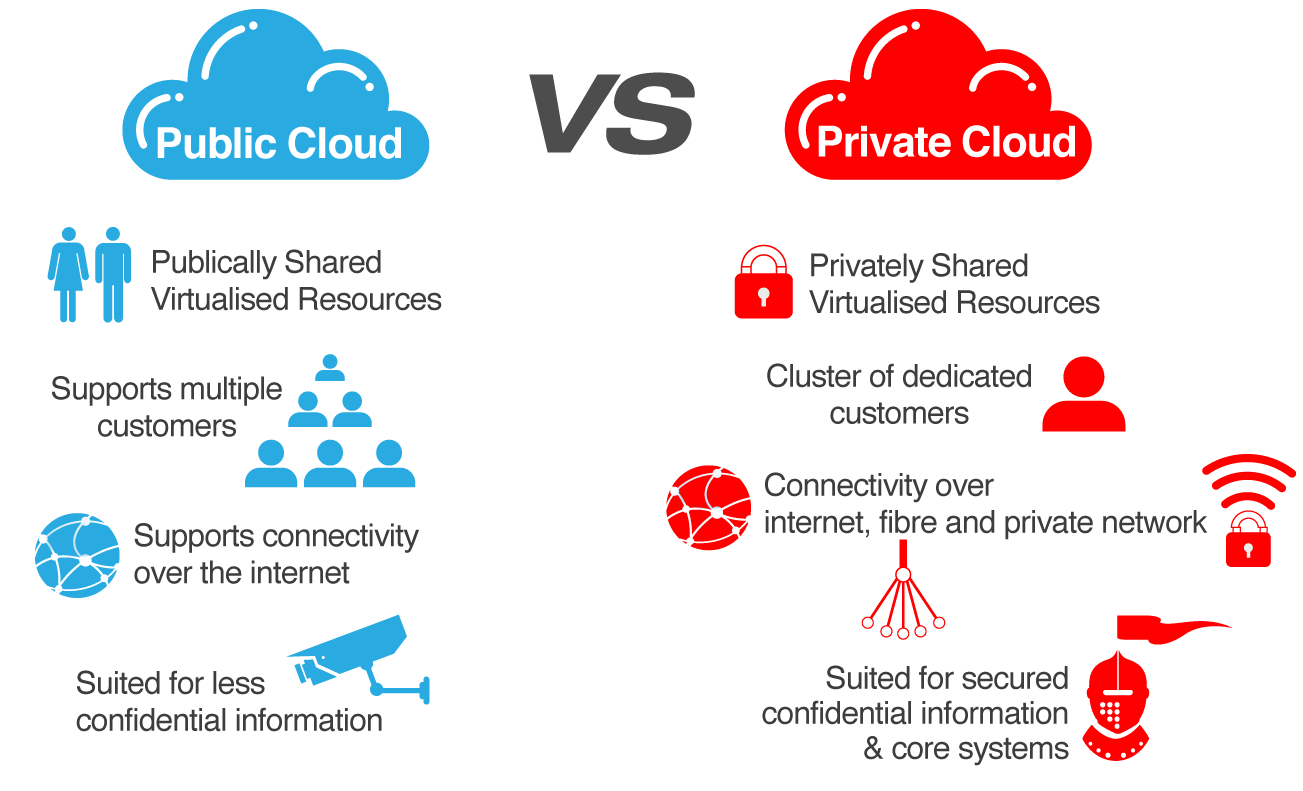
\includegraphics[width=0.55\textwidth]{img/privatePublic.png}
    \caption{Comparações entre nuvem pública e privada}
\end{figure}

\subsection{Nuvem híbrida}

A nuvem híbrida usa uma base de nuvem privada combinada ao uso estratégico de 
serviços de nuvem pública~\cite{ibm-what-is-cloud-computing}. A realidade é que uma 
nuvem privada não pode existir isolada do restante dos recursos de TI e a nuvem 
pública de uma empresa. A maioria das empresas com nuvens privadas se desenvolverão 
para gerenciar cargas de trabalho entre data centers, nuvens privadas e nuvens 
públicas --- criando, assim, nuvens híbridas~\cite{ibm-what-is-cloud-computing}.

Nas nuvens híbridas, há uma composição dos modelos de nuvens públicas e privadas.
Essa característica possui a vantagem de manter os níveis de serviço mesmo que
haja flutuações rápidas na necessidade dos recursos~\cite{technet-cloud-computing}.
A conexão entre as nuvens pública e privada pode ser usada até mesmo em tarefas
periódicas que são mais facilmente implementadas nas nuvens públicas, por
exemplo~\cite{technet-cloud-computing}.

O fator chave para o sucesso da nuvem híbrida: a capacidade para gerenciar de
forma eficiente e segura a combinação de serviços de nuvem pública e privada
como um único ambiente de computação unificado, tirando proveito integral da
nuvem~\cite{ibm-what-is-cloud-computing}.

\subsection{Nuvem comunitária}

Na nuvem comunitária, a infraestrutura de nuvem é compartilhada por diversas 
organizações e suporta uma comunidade específica que partilha preocupações (por 
exemplo, a missão, os requisitos de segurança, política e considerações sobre o 
cumprimento)~\cite{brown2014seguranca}. Pode ser administrado por organizações ou 
por um terceiro e pode existir localmente ou remotamente~\cite{brown2014seguranca}.

% \begin{figure}[ht]
%     \centering
%     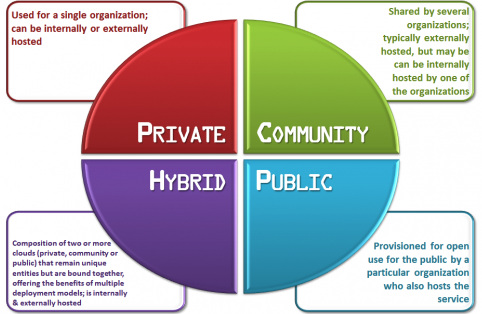
\includegraphics[width=0.65\textwidth]{img/modelosNuvem.png}
%     \caption{Características principais de cada modelo}
% \end{figure}

\chapter{Gerenciamento da segurança da informação na nuvem}

Para a segurança de uma rede em nuvem, devem-se sempre seguir os princípios abaixo:

\newcommand{\itemm}[1]{\item\textbf{#1}}

\begin{itemise}

    \itemm{Acesso privilegiado de usuários}: A sensibilidade de informações
    confidenciais nas empresas leva a um controle de acesso dos usuários e
    informação bem específica de quem terá privilégio de administrador.
    
    \itemm{Conformidade com regulamentação}: As empresas são responsáveis pela
    segurança, integridade e a confidencialidade de seus próprios dados. Os
    fornecedores de computação em nuvem devem estar preparados para auditorias
    externas e certificações de segurança.
    
    \itemm{Localização dos dados}: A empresa que usa uma nuvem provavelmente não
    sabe exatamente onde os dados estão armazenados, talvez nem o país onde as
    informações estão guardadas. O fornecedor deve estar disposto a se comprometer a
    armazenar e a processar dados em jurisdições específicas, assumindo um
    compromisso em contrato de obedecer os requisitos de privacidade que o país de
    origem da empresa pede.
    
    \itemm{Segregação dos dados}: Geralmente uma empresa divide um ambiente com
    dados de diversos clientes. Com isso, surge a necessidade de separação de dados,
    aplicando-se criptografia.
    
    \itemm{Recuperação dos dados}: O fornecedor da nuvem deve saber onde estão os
    dados da empresa e o que acontece para recuperação de dados em caso de
    catástrofe. Qualquer aplicação que não replica os dados e a infraestrutura em 
    diversas localidades está vulnerável para falha completa. Torna-se importante
    ter um plano de recuperação e um tempo estimado para tal.
    
    \itemm{Apoio à investigação}: A existência de atividades ilegais pode se tornar
    impossível na computação em nuvem, uma vez que há uma variação de servidores
    onde estão localizados os acessos e os dados dos usuários conforme o tempo.
    
    \itemm{Viabilidade em longo prazo}: No mundo ideal, o fornecedor de computação
    em nuvem jamais vai falir ou ser adquirido por uma empresa maior. A empresa
    precisa garantir que os seus dados estarão disponíveis caso o fornecedor de
    computação em nuvem deixe de existir ou seja migrado para uma empresa maior.
\end{itemise}
\undef\itemm

De forma a diminuir o impacto de falhas na segurança, devem-se sempre considerar os
possíveis riscos:
\begin{itemise}
    \item Impacto prejudicial advindo do manuseio inadequado de dados.
    \item Encargos por serviços não autorizados.
    \item Problemas financeiros ou legais do fornecedor.
    \item Problemas operacionais ou encerramentos do fornecedor.
    \item Problemas de recuperação de dados e confidencialidade.
    \item Preocupações gerais com segurança.
    \item Ataques de sistema por forças externas.
\end{itemise}

Com o uso de sistemas na nuvem, há o risco sempre presente da conectividade,
segurança de dados e ações dolosas interferindo com os processos de computação.
Entretanto, com um plano bem pensado, uma metodologia para selecionar o provedor
de serviço e uma perspectiva astuta do gerenciamento de risco em geral, a maioria
das empresas pode usar essa tecnologia com segurança. 

\section{Pesquisas do Gartner}


\subsection{Estudos gerais}

A seguir, apresentamos alguns estudos do Gartner (líder mundial na
pesquisa de tecnologia de informação que também atua como empresa de consultoria):

\begin{itemise}

    \item Aproximadamente 19\% das organizações ao redor do mundo estão utilizando a
    computação em nuvem para produção de aplicações, enquanto outros 20\% contratam
    serviços públicos de armazenamento na nuvem. O principal modelo sendo utilizado é
    a da nuvem híbrida~\cite{gartner-public-cloud-services}.

    \item Consumidores armazenarão mais de 1/3 de seu conteúdo digital na nuvem por
    volta de 2016~\cite{gartner-one-third}.

    % Segundo estimativas do grupo americano de informática IBM, o mercado mundial de
    % computação em nuvem poderia alcançar os 200 bilhões de dólares em 2020.

\end{itemise}

Os resultados mostram que a nuvem oferece grandes oportunidades de negócios,
especialmente para serviços de armazenamento. 

Ao mesmo tempo, a indústria de serviços de nuvem é grande e conta com muitos 
provedores com estratégias agressivas para conquistar clientes. Para orientar as 
companhias na hora de selecionar seu parceiro, o Gartner elegeu os dez principais 
fornecedores de serviços de armazenamento~\cite{gartner-top-10}, levando em 
consideração a capacidade deles de atendimento aos clientes:

\begin{figure}[ht]
    \centering
    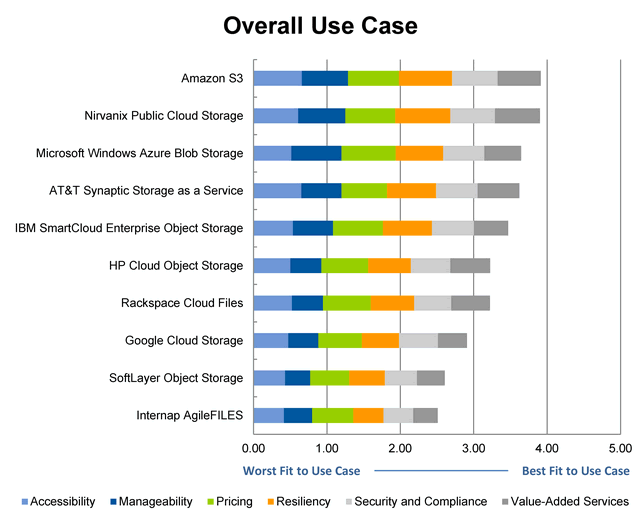
\includegraphics[width=0.8\textwidth]{img/top10.png}
    \caption{Avaliação dos dez principais fornecedores, segundo o Gartner}
\end{figure}


\subsection{Os 10 maiores mitos sobre a nuvem}

Mesmo com uma definição formal a qual muitos concordam, várias perspectivas ainda
contribuem para mistificar a computação em nuvem. Somado à propaganda incessante,
a confusão resultante permeia a área de TI e além nos dias atuais. No final de 2014,
o Gartner destacou 10 dos mitos mais perigosos e enganadores sobre a nuvem:

    \subsubsection{A nuvem está sempre ligada ao capital}

    Apesar dos preços estarem caindo, especialmente para os IaaS, nem todos os
    serviços de nuvem estão ficando mais baratos. Assumindo que a nuvem sempre traz
    benefícios econômicos pode levar a limitações na carreira. Economizar capital
    pode ser um dos benefícios, mas não é sempre uma certeza.

    \subsubsection{Você precisa estar na nuvem para ser bom}

    Organizações de TI estão cada vez mais usando serviços de nuvem como parte de
    suas tentavias de ganhar finanças e atingir demandas e estratégias da nuvem. O
    mito resultante é que as pessoas estão caindo na armadilha de acreditar que, se
    algo é bom, então precisa estar na nuvem.

    \subsubsection{A nuvem deve ser usada para tudo}

    Relacionada ao mito 2, este se refere à crença de que as características reais da
    nuvem se aplicam, ou são desejadas, para tudo. Claramente, há alguns casos de uso
    onde funcionam bem, mas nem todas as aplicãções se beneficiam da nuvem. A menos
    que haja redução de custos, mover uma aplicação legada imutável não é uma boa
    ideia.

    \subsubsection{"Mas o diretor executivo disse" é uma estratégia de nuvem}

    Quando perguntados sobre qual a sua estratégia de nuvem, muitas companhias, por
    não terem uma, costumam dizer que só estão fazendo o que o CEO (diretor
    executivo) quer. Isto não é uma estratégia de nuvem. Esta começa com a 
    identificação de objetivos de negócio e o mapeamento de benefícios em potencial
    da nuvem, ao mesmo tempo em que as inconveniências são atenuadas. A nuvem deve
    ser considerada como um meio para um determinado fim, que deve ser primeiramente
    especificado.

    \subsubsection{Nós precisamos de uma estratégia ou fornecedor de nuvem}

    Serviços de nuvem são vastos, com diversas camadas (IaaS, SaaS...) e aplicações.
    Uma estratégia de nuvem deve ser baseada em alinhar os objetivos de negócio com
    benefícios em potencial. Tais objetivos e benefícios são diferentes em vários
    casos de uso e devem guiar as atividades comerciais, ao invés de servirem como
    tentativas de uniformizar uma oferta ou estratégia.

    \subsubsection{A nuvem é menos segura do que recursos instalados localmente}

    Computação em nuvem às vezes é vista como algo não tão seguro. Isso é mais um
    problema de confiança do que baseado em uma análise razoável de capacidades de
    segurança. Até pelo menos 2014 (data em que a pesquisa fora feita), houve poucas
    falhas de segurança na nuvem pública --- a maioria dos problemas ocorrem em
    recursos locais em ambientes de data center. Apesar dos fornecedores de nuvem
    possuírem o dever de demonstrar suas capacidades, quando isso é feito não há
    razão para desconfiar da segurança de suas ofertas.

    \subsubsection{A nuvem não deve ser usada para casos de risco}

    Computação em nuvem não é "tudo ou nada". Ela está sendo adotada aos poucos e em
    casos específicos. Portanto, não é de se surpreender que casos de uso iniciais
    geralmente não são para sistemas críticos. No entanto, muitas organizações
    progrediram além dos casos de usos iniciais e experimentãção, e estão usando a
    nuvem para tarefas críticas. Há também muitas empresas (não apenas pequenas
    \emph{startups}) que "nascem na nuvem" e possuem todo o seu negócio (claramente
    de sistemas críticos) completamente na nuvem.

    \subsubsection{Nuvem = Data center}

    A maioria das decisões de nuvem não são (e não deveriam ser) sobre fechar
    completamente data centers e mover tudo para a nuvem. Uma estratégia de nuvem
    também não deve ser comparada a uma estratégia de data center. É necessário haver
    espaço de data center para dados que não estão na nuvem e, se forem retirados do
    data center, haverá consequências. Em resumo, nuvem e data center não são
    sinônimos.

    \subsubsection{Migrar para a nuvem leva ao ganho de todas as suas
                   características}

    Não se deve assumir que "migrar para a nuvem" levará à herança de todas as
    características da nuvem vindas de níveis mais baixos (como IaaS). Os atributos
    da nuvem não são transitivos; deve-se distinguir aplicações oferecidas na nuvem
    dos serviços de nuvem em si. Há alguns pontos da nuvem que trazem benefícios,
    como não haver necessidade de comprar hardware, mas tais pontos não levam aos
    mesmos resultados.

    \subsubsection{Virtualização = Nuvem privada}

    Virtualização é uma tecnologia comumente usada em computação em nuvem. No
    entanto, não é a única maneira de se implementar uma nuvem, nem é suficiente
    para tal implementação. Isto é relevante em discussões de nuvem privada, onde
    ambientes altamente virtualizados e automatizados são comuns; em muitos casos,
    é exatamente o que é necessário. Infelizmente, tais ambientes são erroneamente
    descritos como "nuvens privadas".

\begin{frame}{Conclusão}
    A ideia não é necessariamente nova, pois já existem serviços que, de certa
        forma, estão dentro do conceito de computação em nuvem:
    \begin{itemise}
        \item<2-> E-mail (Gmail e Yahoo! Mail)
        \item<3-> Discos virtuais (Dropbox ou OneDrive)
        \item<4-> Armazenamento e compartilhamento de fotos ou vídeos (Flickr e
            YouTube)
    \end{itemise}
\end{frame}

\begin{frame}{Conclusão}
    Na prática, para algumas empresas a adoção da nuvem foi mais complicada do que o
        previsto:
    \begin{itemise}
        \item<2-> Os custos de implementação foram mais altos do que o esperado
        \item<3-> A integração dos serviços de nuvem à infraestrutura de tecnologia
            existente foi especialmente difícil
    \end{itemise}
    \uncover<4->{
        Para os pequenos usuários, a tendência é que os computadores do futuro terão
        preços baixos, visto que serão produzidos de forma mais simplificada
    }
\end{frame}



% \section*{Bibliografia}

\clearpage
\printbibliography
\nocite{*}
\addcontentsline{toc}{section}{Referências}


\end{document}
